\documentclass{article} % For LaTeX2e
% We will use NIPS submission format
\usepackage{nips13submit_e,times}
% for hyperlinks
\usepackage{hyperref}
\usepackage{url}
% For figures
\usepackage{graphicx} 
\usepackage{subfigure} 
% math packages
\usepackage{amsmath}
\usepackage{amsfonts}
\usepackage{amsopn}
\usepackage{ifthen}
\usepackage{natbib}

\title{Project-I by Group Sao Paulo}

\author{
Damien Engels\\
EPFL \\
\texttt{damien.engels@epfl.ch} \And No\'emie Jaquier\\
EPFL \\
\texttt{noemie.jaquier@epfl.ch} \\
}

% The \author macro works with any number of authors. There are two commands
% used to separate the names and addresses of multiple authors: \And and \AND.
%
% Using \And between authors leaves it to \LaTeX{} to determine where to break
% the lines. Using \AND forces a linebreak at that point. So, if \LaTeX{}
% puts 3 of 4 authors names on the first line, and the last on the second
% line, try using \AND instead of \And before the third author name.

\nipsfinalcopy 

\begin{document}

\maketitle

\begin{abstract}
In this report, ...
\end{abstract}

\section{Data Description}
Our train-data consists of ...

\section{Data visualization and cleaning}
We performed basic exploratory data analysis on our data. Figure \ref{fig:boxplotX} ...

\begin{figure}[!h] % !t
\center
\subfigure[Boxplot of real-valued $\mathbf{X}$. Data is not centered and therefore we normalize it.]{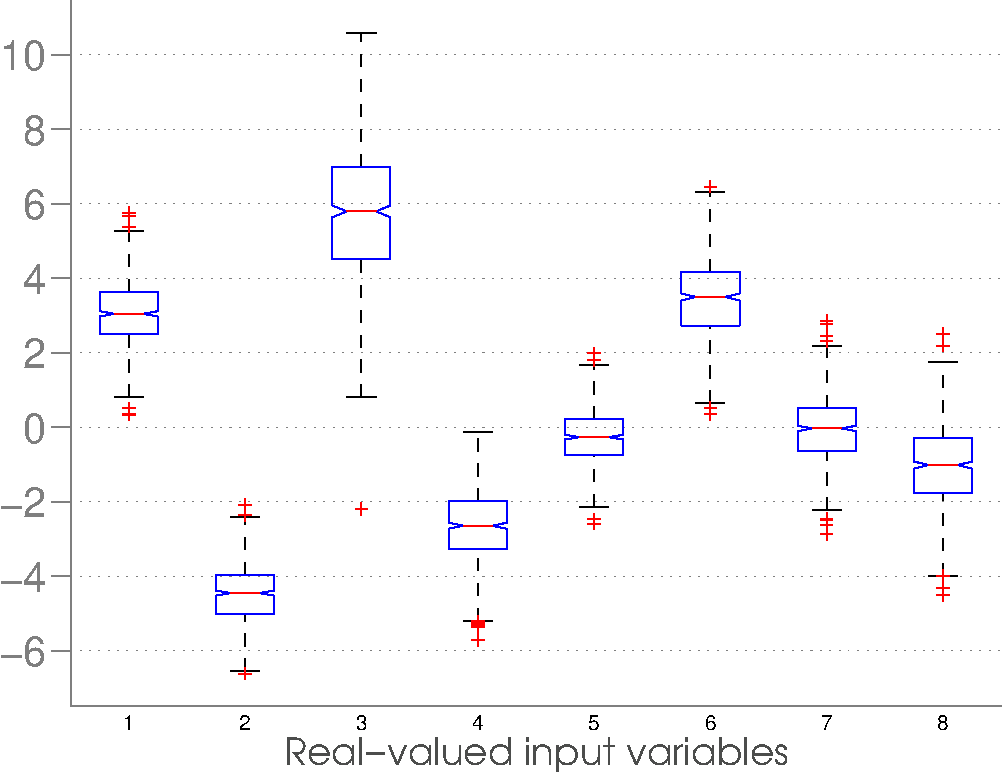
\includegraphics[width=2.5in]{figures/boxplotX.pdf} \label{fig:boxplotX}}
\hfill
\subfigure[Histogram of $\mathbf{y}$. We can clearly see two outliers.]{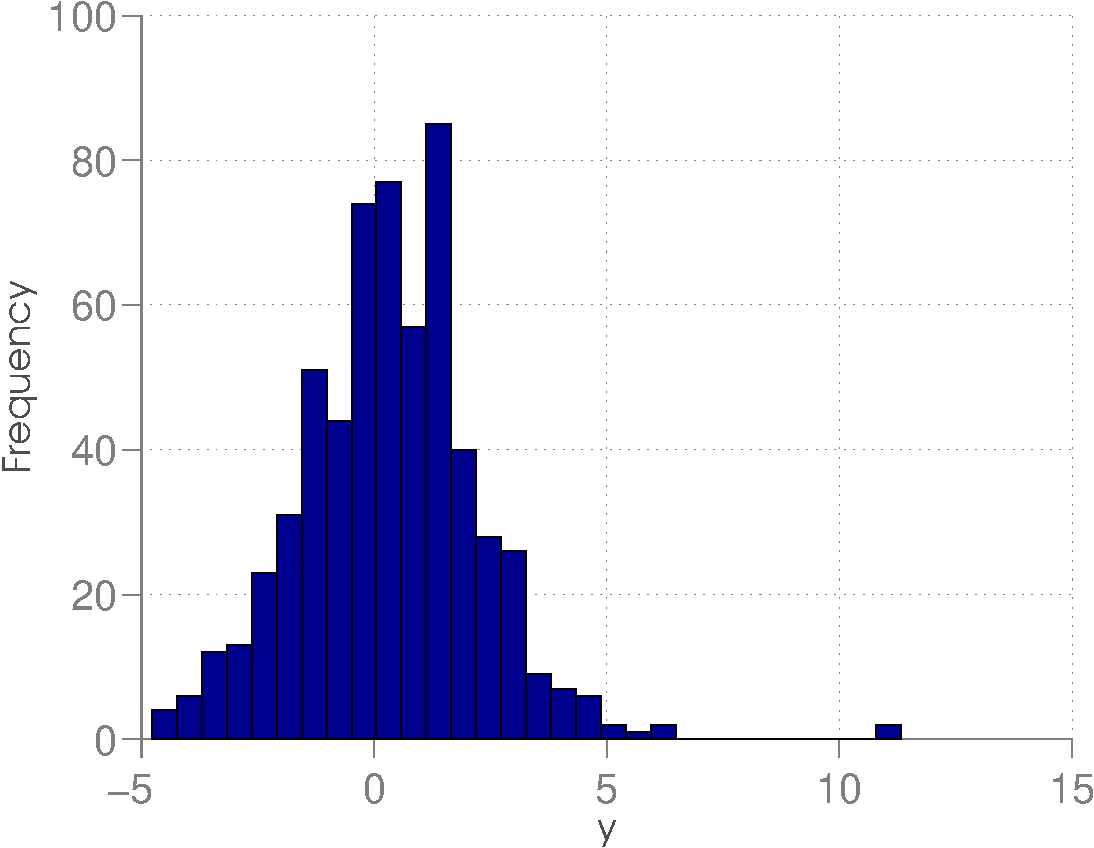
\includegraphics[width=2.5in]{figures/histY.pdf} \label{fig:histY}}
\caption{}
\end{figure}

\section{Ridge regression}
We applied least-squares and ridge regression to this dataset...

\section{Feature transformations}
We tried several feature transformations...


\section{Summary}
In this report, we ...


\subsubsection*{Acknowledgments}
...

\subsubsection*{References}

\end{document}
